
\chapter{Arquitetura de Software}
\label{sec-arquitetura}
\vspace{-1cm}

A Figura~\ref{figura-arquitetura} mostra a arquitetura do sistema \emph{\imprimirtitulo}.

\begin{figure}[h]
	\centering
	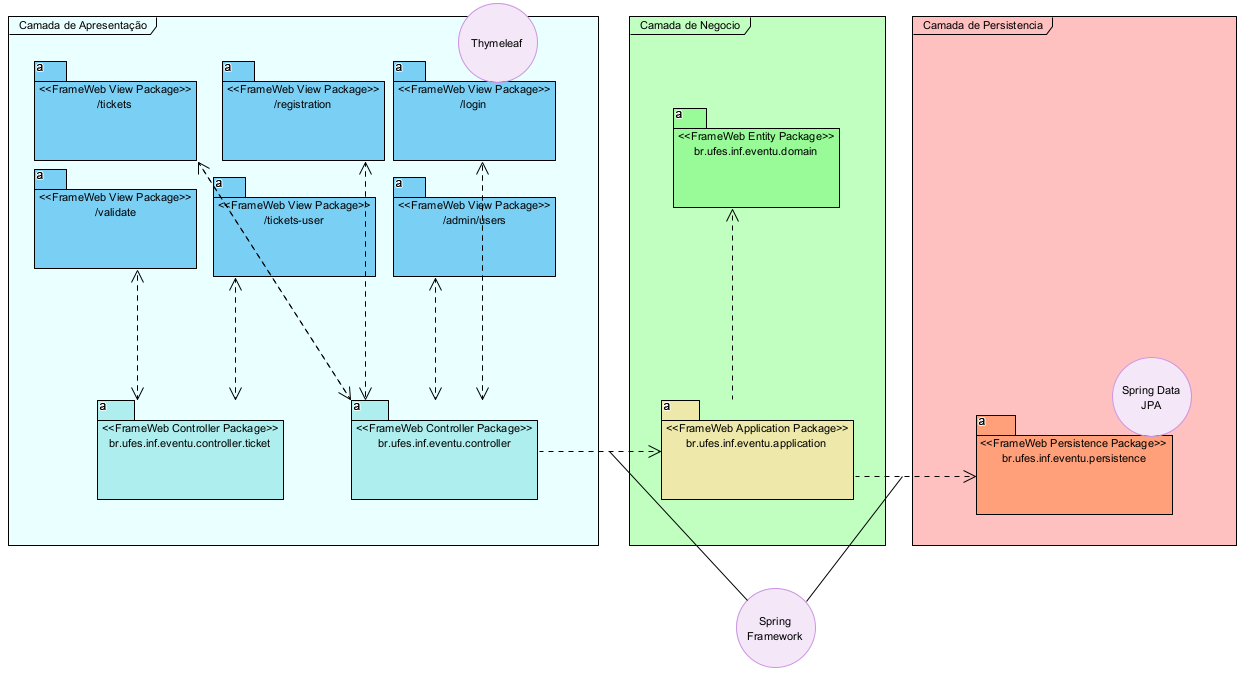
\includegraphics[width=0.8\textwidth]{figuras/Arquitetura.PNG}
	\caption{Arquitetura de Software.}
	\label{figura-arquitetura}
\end{figure}

O sistema \emph{\imprimirtitulo} adota a arquitetura Model-View-Controller (MVC)\cite{fowler:book02} para prover organização, modularidade e separação de conceitos (do inglês \textit{separation of concerns}, SoC). Além disso, a escolha da arquitetura MVC torna-se prática, dado o grande suporte que o framework Spring provê à esta arquitetura.

O sistema \emph{\imprimirtitulo} implementa cada um dos módulos MVC da seguinte forma:

\textbf{Modelo}: No núcleo do sistema, o Modelo encapsula os dados e regras de negócio, gerenciando o acesso e a manipulação de informações sobre eventos, palestrantes, participantes e inscrições. Nele estão os pacotes do modelo de aplicação (ex: ManageAttractionServiceImpl, AuthenticateUserServiceImpl), classes de dominio (ex: Ticket, User, Attraction) e de persistencia (ex: TicketJPADAO, UserJPADAO)

\textbf{Visão}: Representado pelas visualizações geradas por templates Thymeleaf e Tailwind CSS, a camada de Visão apresenta os dados do Modelo para os usuários, permitindo visualização, interação e manipulação de informações.

\textbf{Controlador}: O Controlador atua como intermediário, recebendo requisições do usuário, fazendo validação dos dados de entrada e direcionando-as para o Modelo e recuperando os dados processados para apresentá-los na Visão. As classes TicketController e UserController fazem parte da camada Controlador.